\subsection{Thrust}

The function \texttt{combnthrust()} accepts the same input arguments as the original function \texttt{combn()} from the CRAN package. \texttt{combnthrust()} can also handle the same types of valid inputs (see Section 2.1).\\
\null
Usage:\\
\null

\texttt{combnthrust <- function(x, m, fun = NULL, simplify = TRUE, ...)}\\
\null

where \texttt{x} is the input vector of integers and/or characters, \texttt{m} is number of elements per combination
\texttt{fun} is the function to be applied to the resulting output, \texttt{simplify} indicates whether the output must be printed as a matrix (set to \texttt{TRUE}) or as a list (set to \texttt{FALSE}), and \texttt{...} are the parameters for \texttt{fun}.\\

\null
Code highlights:\\
\begin{itemize}
\item We followed this tutorial \cite{matlofftutorial} to link Rcpp, Thrust, and C++.
\item We used Thrust's  for\_each function to call on the functor that finds the combination for each element, up to \texttt{n - m + 1} in a parallel manner. 
\end{itemize}
Other notes:
\begin{itemize}
\item The program terminates if Thrust is unable to allocate enough space on the GPU to have the program run successfully. 
\item Since Thrust calls are CUDA kernel calls, there is some latency involved in this, which slows the program down. 
\item Thrust uses shared memory because the CUDA backend utilizes the GPU and GPUs have shared memory. 
\end{itemize}


\subsubsection{Comparative Analysis}
The same input sizes and function arguments as in Section 3.1.5 were used for testing Thrust. The following plot illustrates the differences in speeds between the Thrust and CRAN implementations:\\
\null

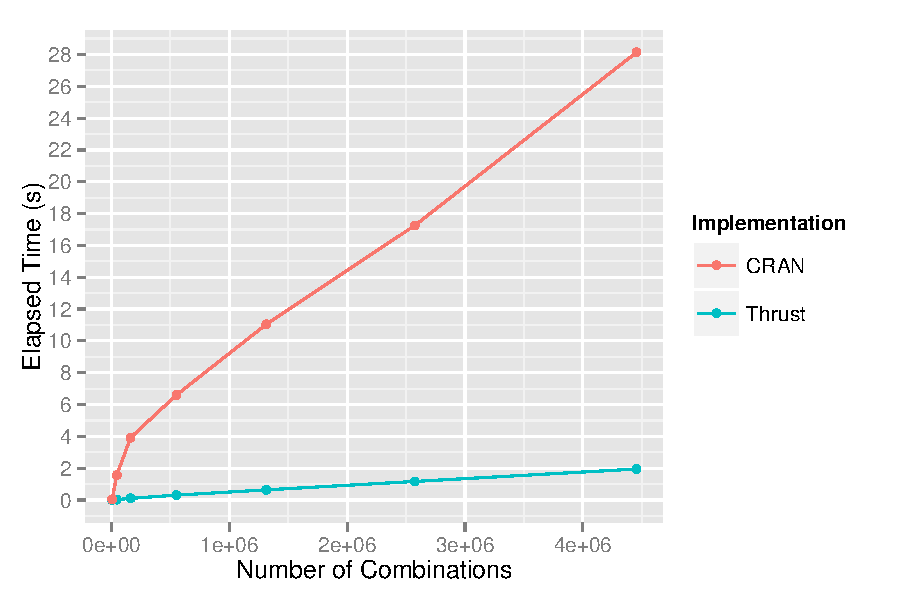
\includegraphics{thrust.pdf}\\
\null

We were able to achieve speedup when using Thrust over the CRAN implementation for smaller input sizes of less than 600. Although the program terminated if the GPU could not allocate enough memory for large input sizes, Thrust was consistently faster than CRAN by using a functor. The program also modified the elements of the output matrix in parallel by making sure the indices didn't conflict. 
